\chapter{Aspects procédés des traitements thermochimiques}
\label{ch:aspects_procedes}

\vfill

Ce chapitre vise à introduire le sujet et à présenter un état de l'art des traitements thermochimiques par transfert de carbone et d'azote dans les aciers faiblement alliés. Une attention particulière sera accordée à la carbonitruration, procédé utilisé il y a plusieurs décennies avec la cémentation et d'autres procédés de durcissement de surface pour améliorer le comportement mécanique de pièces d'ingénierie~\cite{Slycke1981i}. Pour cela, la Section~\ref{sec:procedes} décrira les principes sous--jacents au contrôle des procédés thermochimiques permettant l'enrichissement en éléments interstitiels comme le carbone et l'azote. Ensuite, les lois de la diffusion à l'état solide et le logiciel Thermo-Calc~\cite{Andersson2002,Borgenstam2000} qui est utilisé pour la simulation des profils de diffusion--précipitation dans les alliages étudiés seront présentés Section~\ref{sec:diffusion}. Les bases de données du logiciel Thermo-Calc~\cite{Andersson2002,Borgenstam2000} contiennent les informations nécessaires aux simulations, \emph{i.e.} des polynômes pour la représentation des propriétés thermodynamiques et de transport. La Section~\ref{sec:dynamique} présente les fondements théoriques requis pour comprendre le couplage hydrodynamique--cinétique qui a lieu au sein des réacteurs réels employés pour des traitements thermochimiques. Finalement, la Section~\ref{sec:cinetique} contiendra les fondements de cinétique chimique selon la loi d'action de masse, ainsi que la méthode de simplification du mécanisme établi afin d'obtenir un nombre réduit d'espèces pour obtenir un modèle moins exhaustif mais plus rapide pour la simulation des écoulements réactifs ayant lieu dans les procédés. 

\vfill\clearpage

\section{Contrôle des procédés thermochimiques gazeux}
\label{sec:procedes}

L'objectif recherché en réalisant des traitements thermochimiques des matériaux métalliques est de transférer des atomes provenant du milieu extérieur à la surface des pièces à partir de réactions hétérogènes~\cite{Gantois2010} et de modifier, dans le cas de la carbonitruration, ses caractéristiques mécaniques. La maîtrise d'un procédé thermochimique comprend l'étude de la cinétique et de la thermodynamique du milieu permettant l'enrichissement de l'interface avec le matériau traité où ont lieu diffusion et transformations métallurgiques.  Cela revient à devoir traiter~\cite{Dulcy2007} le transport des espèces réactives en phase gazeuse vers la surface de l'acier, ce qui inclut la cinétique chimique, la diffusion dans le gaz et l'hydrodynamique du système, les réactions physicochimiques et chimiques à la surface de l'acier et le transport à l'état solide \textendash{} diffusion-précipitation \textendash{} des atomes incorporés par réaction hétérogène. Cet ensemble de phénomènes doit être pris en compte pour simuler le procédé thermochimique au moyen des équations: 
\begin{itemize}
  \item de bilan matière dans le gaz, à l'interface et dans le solide, 
  \item de conservation de la quantité de mouvement et des espèces, 
  \item de transport de la chaleur et de la diffusion de matière.
\end{itemize}

\begin{figure}[h]
  \centering{}
  \resizebox{0.9\textwidth}{!}{%
    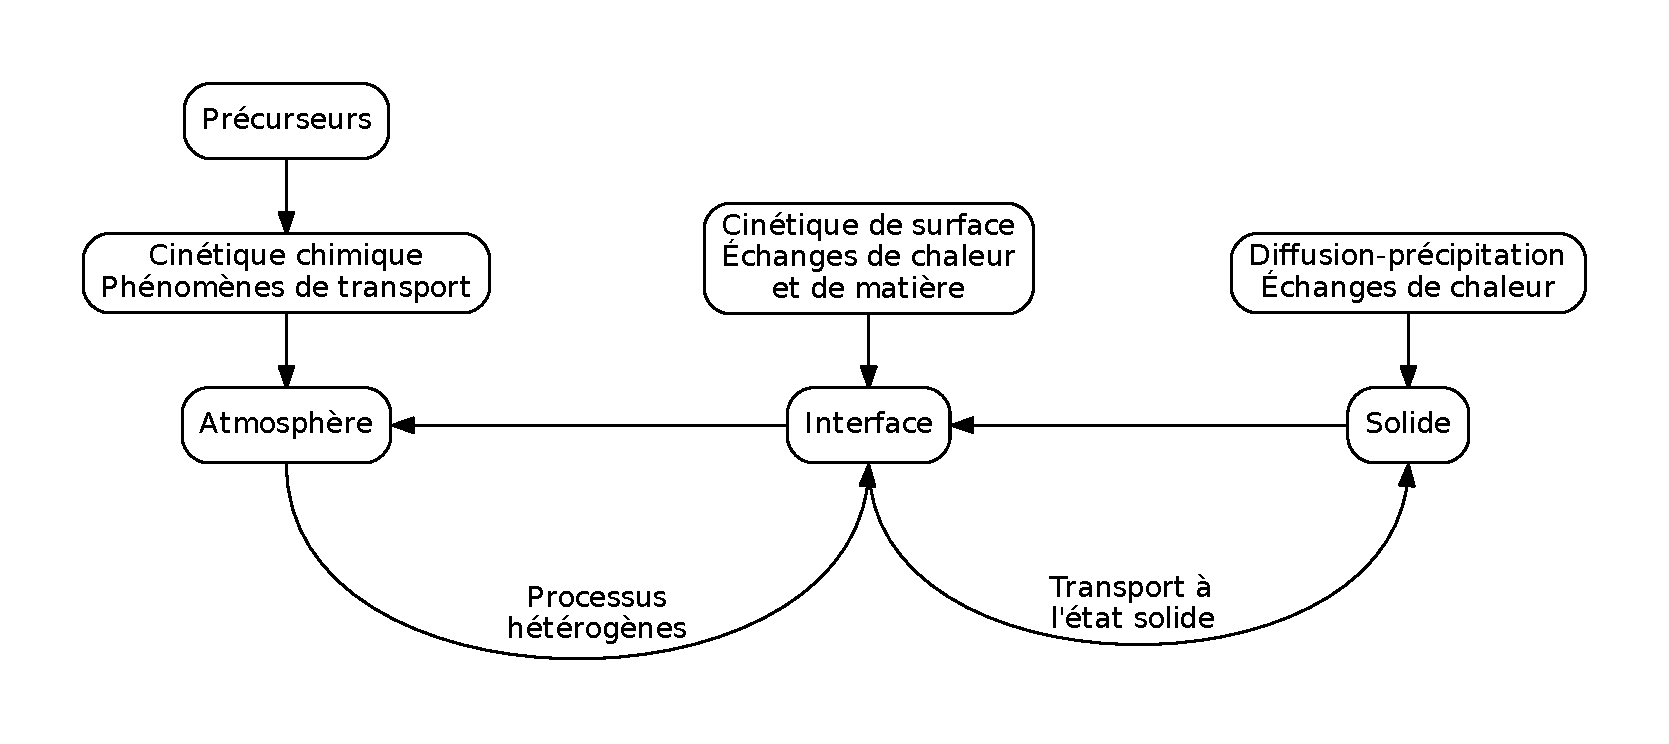
\includegraphics{figures/ch-01-schema-traitements}}
  
  \caption{\label{fig:schema-traitements}Schéma illustrant les principaux processus ayant lieu dans les différentes régions utilisées pour décrire les traitements thermochimiques gazeux.}
\end{figure}

Plusieurs simplifications qui peuvent être mises à profit pour l'optimisation des procédés sont possibles selon le comportement cinétique de l'atmosphère de traitement. Cela peut être illustré, par exemple, dans le cas où l'atmosphère atteint rapidement l'équilibre, cas pour lequel il n'y a pas de couplage entre cinétique et hydrodynamique : l'enrichissement des surfaces peut alors être simplement contrôlé en connaissant l'équilibre gaz--solide. Une autre simplification est possible si l'établissement d'un état stationnaire en phase gazeuse pour un débit donné a lieu. On peut alors considérer un pseudo--équilibre à l'interface gaz--solide. Comme ce travail aborde la carbonitruration comme une série d'étapes successives de cémentation et de nitruration, les discussions sur le contrôle des atmosphères carburantes et nitrurantes se feront séparément. \citet{Slycke1981i} ont abordé l'enrichissement simultané en carbone et en azote.

\subsection{Contrôle de l'étape de cémentation}
\label{sec:controle_cementation}

Le temps caractéristique pour atteindre l'équilibre des atmosphères \ch{CO-H2} dans la plage de température typiquement employée pour la carbonitruration  est court par rapport à la durée de traitement~\cite{Yahia1995,Dulcy2007}. Dans ce cas, l'enrichissement en carbone est indépendant de l'écoulement si le débit total des gaz précurseurs est suffisant pour permettre un enrichissement avec une condition aux limites à concentration constante à l'état stationnaire.  Si ces conditions ne sont pas atteintes, la consommation du carbone disponible dans l'atmosphère est plus rapide que l'arrivée du gaz et une condition à flux variable s'établit. Les paramètres pour établir ce type de contrôle dépendent du volume du four, de la surface totale des pièces traitées, du système de circulation de gaz, etc~\cite{Dulcy2007}. Cette hypothèse d'équilibre permet d'utiliser le potentiel carbone comme paramètre de contrôle du procédé, paramètre dont la définition la plus simple et générale est \og{}\textit{le potentiel carbone d'une atmosphère est la fraction massique en carbone d'un acier en équilibre thermodynamique avec cette atmosphère}~\cite{Dulcy2007}{}\fg.  Cette grandeur, notée $P_{C}$ dans sa représentation en pourcentage massique, est caractéristique de l'atmosphère et n'a de sens que si le système est en équilibre.  À partir des expressions de l'équilibre gaz--solide, on calcule l'activité du carbone dans le matériau. Pour cela, on prend comme état de référence le graphite, comme cela est fait dans l'Équation~\ref{eq:ellis_carbone}~\cite{Dulcy2007}.

\begin{equation}
  a_{C}^{m}=1,07\cdotp Q\cdotp\left(\frac{\si{\%}P_{C}}{100-19,6\si{\%}P_{C}}\right)
    \cdotp\exp\left(\frac{4798,6}{T}\right)
  \label{eq:ellis_carbone}
\end{equation}

Dans cette Équation~\ref{eq:ellis_carbone} le paramètre $Q$ est une fonction de la composition de l'acier et sert à introduire l'influence des éléments d'alliage dans le calcul de l'équilibre entre la fraction massique en carbone dans le matériau et l'activité correspondante dans le gaz. Une des expressions disponibles dans la littérature pour son calcul est fournie par \citet{Gunnarson1967} et est donnée par l'Équation~\ref{eq:gunnarson}.
\begin{equation}
  \begin{split}
  Q=1 & +\si{\%}\ch{Si}\left(0,15+0,033\si{\%}\ch{Si}\right)-0,0365\si{\%}\ch{Mn}
        -\si{\%}\ch{Cr}\left(0,13-0,0055\si{\%}\ch{Cr}\right)\\
      & +\si{\%}\ch{Ni}\left(0,03+0,00365\si{\%}\ch{Ni}\right)
        -\si{\%}\ch{Mo}\left(0,025+0,01\si{\%}\ch{Mo}\right)
  \end{split}
  \label{eq:gunnarson}
\end{equation}

Plusieurs expressions d'équilibre peuvent être écrites pour les atmosphères à base de \ch{CO - H2}. Le choix de l'équilibre considéré pour le réglage du procédé implique la mesure d'une grandeur physique spécifique, ce qui demandera une méthode différente de détection. En général, la mesure de la température du point de rosée, la mesure de la pression partielle d'oxygène ou la mesure par absorption infrarouge de la pression partielle de \ch{CO} sont réalisées dans ce but~\cite{Dulcy2007}. Par exemple, pour un contrôle basé sur la température de point de rosée, l'équilibre en phase gazeuse de la réaction du gaz à l'eau donné par \ch{CO + H2 <=> C_{m} + H2O} et sa constante d'équilibre en termes de pression $K_{p}$ \textendash{} pressions partielles données en \si{\atm} \textendash{} permet d'établir l'expression de l'activité $a_{C}^{g}$ du carbone dans le gaz grâce à l'Équation~\ref{eq:equilibre_point_de_rose}. 

\begin{equation}
  a_{C}^{g}=
  \frac{P\left(\ch{CO}\right)\cdot P\left(\ch{H2}\right)}
  {P\left(\ch{H2O}\right)}\cdot
  \exp\left(\frac{16763}{T}-17,5842\right)
  \label{eq:equilibre_point_de_rose}
\end{equation}

L'hypothèse d'équilibre à l'interface gaz--solide nous permet d'écrire $a_{C}^{m}=a_{C}^{g}$. Cette expression  permet de comprendre les relations entre les paramètres opératoires \textendash{} composition de l'atmosphère et la température \textendash{} et la composition de la nuance traitée \textendash{} en termes du paramètre $Q$ \textendash{} avec la teneur en carbone obtenue en surface \textemdash{} le potentiel carbone $P_{C}$. Pour des alliages différents, la teneur en carbone $P_{C}$ \textendash{} pour une activité constante de l'atmosphère $a_{C}^{g}$ \textendash{} sera d'autant moins importante que la valeur de $Q$ sera élevée. On peut vérifier cela à partir des Équations~\ref{eq:ellis_carbone}~et~\ref{eq:equilibre_point_de_rose} et de la condition d'équilibre $a_{C}^{m}=a_{C}^{g}$ en faisant:

$$
P_{C}=\frac{10000\cdotp{}a_{C}^{m}}{107\cdotp{}Q\cdotp{}{\exp\left(\frac{4798,6}{T}\right)}+1960\cdotp{} a_{C}^{m}}
$$ 

Les Équations~\ref{eq:ellis_carbone}~et~\ref{eq:equilibre_point_de_rose} permettent le calcul de la pression partielle de vapeur d'eau $P\left(\ch{H2O}\right)$ à l'équilibre dans le système. Cette grandeur est utilisée dans l'Équation~\ref{eq:point_rosee} avec la pression de travail $P_{ref}$ du système dans le calcul de la température de point de rosée $T_{r}$ du gaz qui peut être mesurée par des techniques analytiques et permet la mise au point et le suivi du procédé. Cette procédure permet de tracer des diagrammes donnant la température du point de rosée $T_{r}$ en fonction de la fraction massique en carbone pour un alliage spécifique, comme celui de la Figure~\ref{fig:dew_point_iron}.  Les données présentées ont été calculées comme cela est décrit dans cette section et comparées à celles calculées par le logiciel Thermo-Calc~\cite{Andersson2002,Borgenstam2000}, au moyen des bases de données SSUB3 pour l'équilibre en phase gazeuse et TCFE7 pour lier l'activité en carbone à sa fraction massique dans le système \ch{Fe-C}. 

\begin{equation}
T_{r}=\frac{5422,13}{14,7316+\ln\biggr(\dfrac{P_{ref}}{P\left(\ch{H2O}\right)}\biggr)}
\label{eq:point_rosee}
\end{equation}

\begin{figure}[!b]
  \centering
  \resizebox{0.6\textwidth}{!}{
    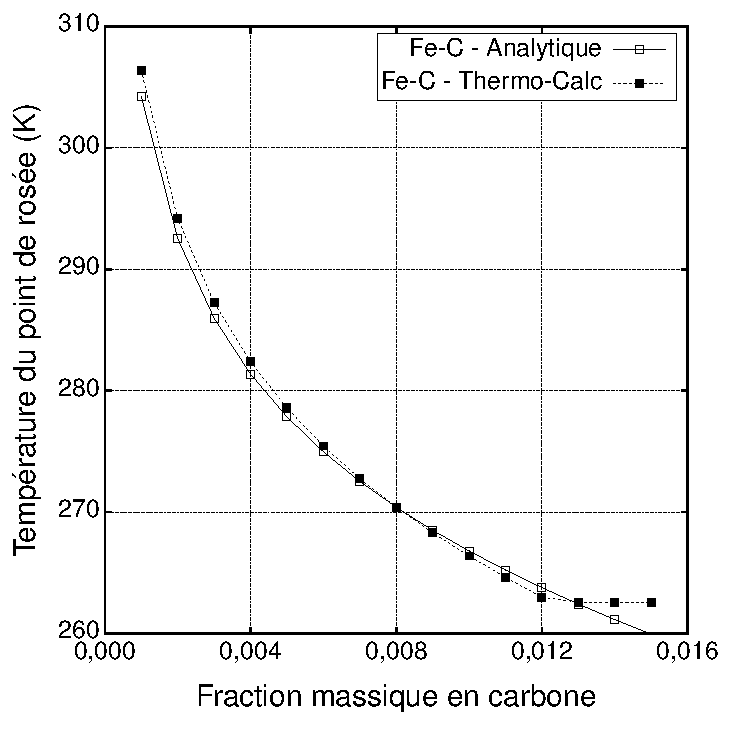
\includegraphics{figures/ch-01-dew_point_iron}}
  
  \caption{\label{fig:dew_point_iron}Température du point de rosée en fonction de la fraction massique en carbone en équilibre avec l'atmosphère pour le système à \SI{1173}{\kelvin}. Atmosphère \ch{N2 - 0,2 H2 - 0,4 CO}.}
\end{figure}

La température de point de rosée requise pour atteindre une fraction massique en carbone visée en surface décroît avec l'augmentation du paramètre $Q$ de l'Équation~\ref{eq:ellis_carbone}. Cela implique donc une pression partielle de l'eau $P\left(\ch{H2O}\right)$ en équilibre avec la surface correspondant à cette teneur en carbone plus faible: plus la fraction en carbone visée en surface est élevée, plus la température du point de rosée associée est faible. La méthode analytique proposée n'est valable que jusqu'à la limite de solubilité en carbone, activité $a_{C}^{m}={1}$. Dans le cas du système binaire \ch{Fe-C}, la fraction massique en carbone dans le matériau devient indépendante de la température du point de rosée $T_{r}$, étant donné qu'il est impossible d'avoir de la diffusion en domaines biphasés dans des systèmes binaires. Cela implique le besoin d'un contrôle précis de $T_{r}$ au voisinage de la limite de solubilité pour limiter la précipitation de cémentite.  Ce n'est pas le cas pour des alliages de fer et des considérations supplémentaires sont alors nécessaires \textemdash{} Section~\ref{sec:classical_carburizing}.

Le contrôle des atmosphères d'hydrocarbures est rapporté par \citet{Yada2013} qui montrent que pour de faibles pressions partielles \textendash{} de l'ordre de \SI{50}{\pascal} \textendash{} il est possible d'atteindre la condition de saturation en surface pour des aciers faiblement alliés. Cependant, les auteurs~\cite{Yada2013} ont réalisé un enrichissement à la saturation en carbone de l'austénite et leurs conditions expérimentales ne sont pas représentatives des réacteurs de grandes dimensions où la décomposition de l'acétylène peut être importante. Cela fait l'objet du Chapitre~\ref{ch:caracterisation_atmospheres} qui traitera des mécanismes de décomposition des hydrocarbures disponibles dans la littérature~\cite{Benzinger1996957,Becker1998177,Becker1998201,Becker1998213, Becker1998225,Norinaga2005,Norinaga2007,Norinaga2007ii,Graf2007,Khan2008, Norinaga2009,Lacroix2010132,Gorockiewicz2011,Fau2013,Ziegler2005107,Ziegler2005212,Ziegler2005231,Ziegler2007268,Ziegler201348} et de leur cinétique, puis du Chapitre~\ref{ch:modelisation_cinetique} pour leur simulation numérique. Autres résultats concernant la cémentation basse pression à partir d'hydrocarbures sont aussi fournis dans la littérature~\citet{Tsuji1987,Liu2003,Iwata2005,Kula2005,Kula201326,Zajusz2014646}.

\subsection{Contrôle de l'étape de nitruration}
\label{sec:controle_nitruration}

La nitruration gazeuse est conduite avec des atmosphères à base d'ammoniac et de ses produits de décomposition~\cite{Slycke1981i,Ginter2006}, comme cela est présenté par la Réaction~\ref{eq:ammonia_hom} et sa constante d'équilibre~\cite{Stolen2004,Landau1980} \textendash{} l'Équation~\ref{eq:ammonia_hom_k} \textendash{} qui vaut $K_{hom}=\SI{1,2E5}{\square\atm}$ à \SI{713}{\kelvin}. Cette valeur montre qu'à cette température, typique pour la nitruration des aciers, l'ammoniac devrait être déjà presque complètement dissocié~\cite{Gantois2010}. Si la température augmente à \SI{1173}{\kelvin}, on obtient $K_{hom}=\SI{2,3E7}{\square\atm}$, valeur qui correspond à une fraction résiduelle en \ch{NH3} de deux ordres de grandeur plus faible que celle disponible typiquement dans la carbonitruration. Selon \citet{Slycke1981i}, cette température impose une limite pratique pour l'enrichissement en azote des aciers faiblement alliés et on ne devrait avoir que du \ch{H2} et du \ch{N2} dans le réacteur. Si l'enrichissement en carbone a lieu en même temps que celui en azote, la fraction résiduelle d'ammoniac ne change pas de façon mesurable~\cite{Slycke1981i}.

\reaction[eq:ammonia_hom]{2 NH3 <=> N2 + 3 H2}

L'Équation~\ref{eq:ammonia_hom_k} devrait permettre de calculer la fraction molaire résiduelle d'ammoniac disponible dans le four pour permettre le transfert de matière vers le solide: ce n'est pas le cas étant donnée la cinétique de décomposition de \ch{NH3}. Selon \citet{Gantois2010} \og\textit{la faible vitesse de dissociation thermique de la molécule de \ch{NH3} en phase gazeuse implique que celle-ci se trouve dans un état de pseudo-équilibre thermodynamique vis-à-vis du temps de séjour relativement court des molécules dans le réacteur, généralement de l'ordre de quelques minutes}\fg{} à la pression atmosphérique. Les temps de séjour dans les traitements thermochimiques à basse pression sont environ de deux ordres de grandeur plus courts. Cela implique que le contrôle du procédé dépend de l'hydrodynamique du réacteur~\cite{Slycke1981i,Ginter2006}, qui impose un temps de séjour moyen des molécules en phase gazeuse dépendant principalement du débit volumique du gaz vecteur~\cite{Gantois2010}.

\begin{equation}
K_{hom}\left(T\right)=
\frac{P\left(\ch{N2}\right)\cdot
  P\left(\ch{H2}\right)^{3}}{P\left(\ch{NH3}\right)^{2}}=
\exp\left[2,3\cdot\biggr(12,392-\frac{5886}{T}\biggr)\right]
\label{eq:ammonia_hom_k}
\end{equation}

Le contrôle du débit des précurseurs permet l'établissement d'une fraction résiduelle constante d'ammoniac dans le gaz. C'est donc cette fraction résiduelle qui doit être en équilibre avec l'azote dans l'acier, comme cela est imposé par la Réaction~\ref{eq:ammonia_het} et sa constante d'équilibre \textendash{} Équation~\ref{eq:ammonia_het_k} \textendash{} \cite{Slycke1981i,Yahia1995}. C'est cette réaction globale avec le solide qui constitue l'étape limitante du procédé dans le cas du fer~\cite{Slycke1981i} et de ses alliages. D'un point de vue élémentaire, l'équilibre précédent est géré par des déshydrogénations successives de l'ammoniac, si bien que l'étape élémentaire limitante dépend des caractéristiques de la surface traitée et bien sûr de la température~\cite{Aparicio1994}.  L'augmentation de la température favorise la formation des produits dans les Réactions~\ref{eq:ammonia_hom}~et~\ref{eq:ammonia_het}, ce qui est mis en évidence par les Équations~\ref{eq:ammonia_hom_k}~et~\ref{eq:ammonia_het_k}, qui présentent des dérivées positives par rapport à la température. Il y a donc une compétition entre l'apport d'azote dans l'austénite et sa décomposition homogène. 

On doit aussi remarquer que l'équilibre introduit des contraintes additionnelles comme la réaction de denitruration \ch{N$^{s}$ <=> 1/2 N2$^(g)$} et peut conduire à la formation de défauts dans la couche: lors de l'interruption de l'apport en \ch{NH3}, le mécanisme de rétro--diffusion d'azote est régi en surface par le processus indirect de la Réaction~\ref{eq:ammonia_het}, ce qui peut provoquer une perte importante de masse. Le procédé peut encore conduire à la formation de gaz \ch{N2} aux joints de grains et autres défauts cristallins où peuvent alors se concentrer ces molécules et promouvoir la formation de porosités. Lorsque des pressions de l'ordre de quelques centaines d'atmosphères s'exercent dans les pores et que les températures sont élevées, la déformation plastique du matériau, associée à la coalescence des pores, conduit à l'apparition de défauts de surface macroscopiques. Les paramètres importants pour la compréhension de la formation de porosité sont donc la température, la durée du traitement et l'activité de l'azote dans l'austénite~\cite{Yahia1995}.  \citet{Yahia1995} observe la formation de porosités dans les échantillons de nuance XC10 avec une fraction massique en azote de 0,006 en surface. Pour les nuances traitées ici, cette teneur doit être plus élevée, dans la mesure où la présence d'éléments d'alliage (principalement le \ch{Cr}) diminue l'activité de l'azote par formation de précipités. Comme cette limite (une fraction massique $w_{N}=0,006$) se situe au-delà de celle définie dans cette étude ($w_{N}=0,004$), la formation importante de porosités n'est pas attendue.
%prévue dans les conditions étudiées.

\reaction[eq:ammonia_het]{NH3 <=>[s] N^s + 3/2 H2}

\begin{equation}
  K_{het}\left(T\right)=
  \frac{a_{N}^{m}\cdot
  P\left(\ch{H2}\right)^{\frac{3}{2}}}{P\left(\ch{NH3}\right)}=
  \exp\left[2,3\cdot\left(6,196-\frac{2943}{T}\right)\right]
  \label{eq:ammonia_het_k}
\end{equation}

C'est à partir de ce pseudo--équilibre que \citet{Lehrer1930} dans les années 1930 a établi pour \ch{Fe-N} un diagramme de phases en fonction d'une grandeur appelée potentiel de nitruration, défini par $K_{N}=\nicefrac{P\left(\ch{NH3}\right)}{P\left(\ch{H2}\right)^{\nicefrac{3}{2}}}= \nicefrac{a_{N}^{m}}{K_{het}}$. Dans cette équation $a_{N}^{m}$, l'activité de l'azote dans l'alliage est une fonction de la teneur en azote $N_{m}$ dans le métal et la relation dépend du modèle de solution adopté. L'équation donnant le $K_{N}$ peut être résolue pour des alliages industriels à l'aide du logiciel Thermo-Calc~\cite{Andersson2002,Borgenstam2000}. Cela permet d'obtenir des diagrammes $K_{N}\text{ vs }N_{m}$ et donc, de déterminer la composition de l'atmosphère permettant d'atteindre la teneur en azote désirée en surface des pièces traitées. La Figure~\ref{fig:diagrammes_kn} présente ces diagrammes pour les alliages étudiés en considérant plusieurs teneurs en carbone et utilisant le diazote à la pression atmosphérique comme état de référence de l'azote \textemdash{} voir Annexe~\ref{an:nitriding-kn}. Il faut prendre en compte le fait que c'est la teneur résiduelle de \ch{NH3} dans l'atmosphère qui permet ce calcul de pseudo--équilibre. D'autres expressions pour décrire l'équilibre gaz--matériau
%, en plus des développements de \citet{Lehrer1930}, 
sont réunies dans une synthèse écrite par \citet{Gantois2010}.

\begin{figure}[!ht]
  \centering
  \subfloat[16NiCrMo13]{
    \centering\resizebox{0.48\textwidth}{!}{
      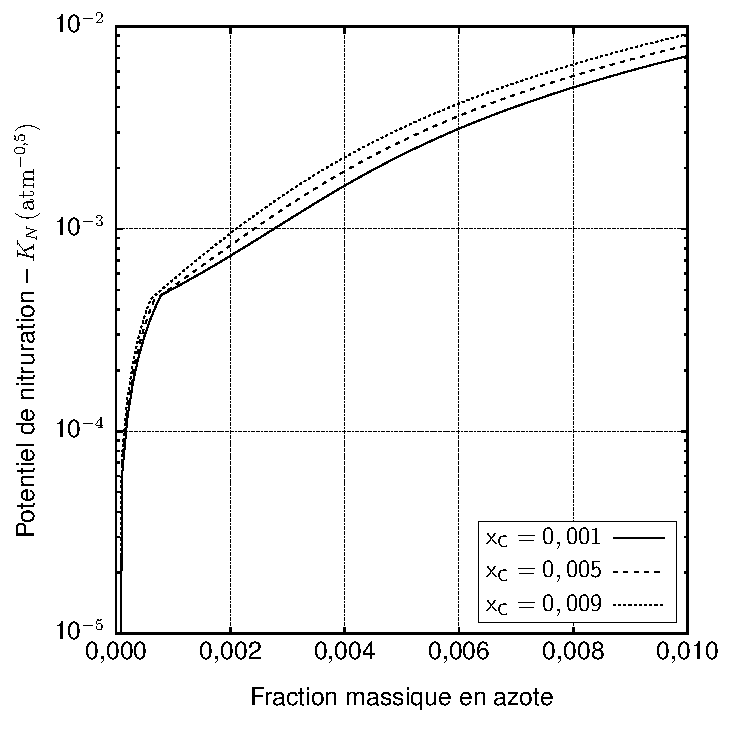
\includegraphics{figures/ch-01-kn_diagram_aero}}
  } \hfill 
  \subfloat[23MnCrMo5]{
    \centering\resizebox{0.48\textwidth}{!}{
      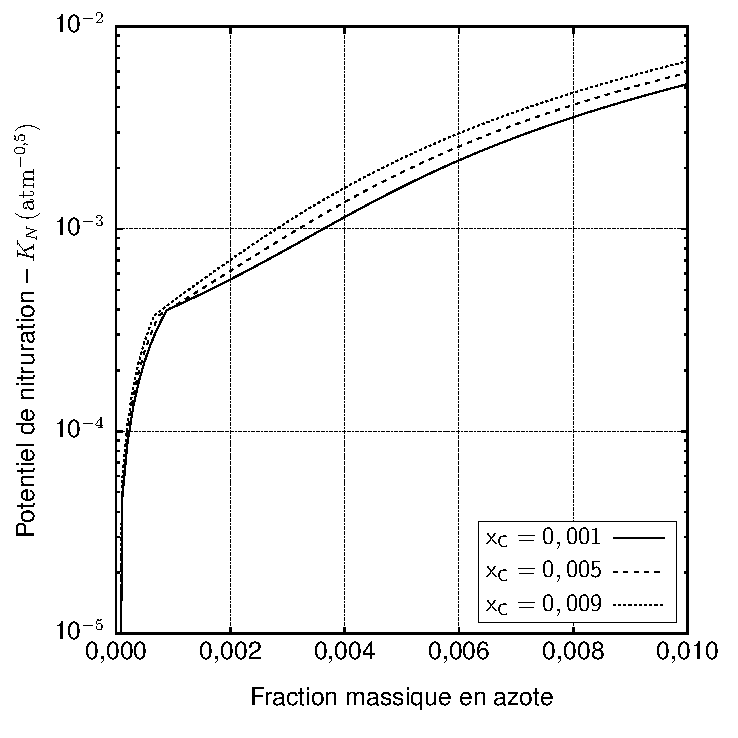
\includegraphics{figures/ch-01-kn_diagram_auto}}
  }

  \caption{\label{fig:diagrammes_kn}Diagrammes donnant le potentiel de nitruration en fonction de la fraction massique en azote en surface dans les alliages 16NiCrMo13 et 23MnCrMo5.}
\end{figure}

\section{Transport de matière à l'état solide}
\label{sec:diffusion}

\subsection{Fondements théoriques}

Le transport de matière à l'état solide est à la base de la majorité des traitements thermochimiques. L'introduction des éléments carbone et azote lors de la carbonitruration se fait à partir d'une réaction de surface entre la pièce et le milieu servant au traitement et ensuite par diffusion de ces éléments vers le c{\oe}ur des pièces traitées~\cite{Slycke1981i}.  Cette migration des atomes se produit par sauts successifs entre les défauts ou espaces vides du cristal sous l'effet de l'agitation thermique.  Si l'on traite la migration des atomes par une méthode statistique, il faut introduire les notions de probabilité de saut, de distance de saut, de directions possibles et de fréquence de vibration atomique~\cite{Jaoul2004}.  Compte tenu de la grande difficulté ou même de l'impossibilité de mesurer ces grandeurs, la définition du coefficient phénoménologique de diffusion $D$ permet, à une échelle beaucoup plus grande que celle de la maille du cristal, de quantifier le flux moyen $J$ de transport de matière.

D'un point de vue physique, c'est le gradient de potentiel chimique $\mu_{i}$, qui est responsable du mouvement atomique conduisant à une augmentation de l'entropie du système~\cite{Guiraldenq1994,Jaoul2004}. Comme il y a proportionnalité entre $\mu_{i}$ et la concentration $c_{i}$ de l'espèce $i$ on établit dans le cas général le flux $J_{i}=-D_{i}\,\vec{\nabla}\cdot{}c_{i}$, ce qui constitue la première Loi de Fick. Le bilan de matière sur ce flux conduit à la seconde loi de Fick, exprimée par l'Équation~\ref{eq:fick_nd}~\cite{Borgenstam2000} dans le cas 1-D. Ces équations régissent la cinétique de transport à l'état solide dans les systèmes simples, comme les mélanges binaires et ne prennent pas en compte des phénomènes de transformation de phases directement.

\begin{equation}
  \frac{\partial c_{i}}{\partial t}=
  \frac{\partial}{\partial x}\biggr(-J_{i}\biggr)=
  \frac{\partial}{\partial x}\biggr(D_{i}\frac{\partial c_{i}}{\partial x}\biggr)
  \label{eq:fick_nd}
\end{equation}

Plus formellement, cette formulation n'est valable que pour des systèmes où le gradient de potentiel chimique, $\nicefrac{\partial\mu}{\partial{}x}$, d'une espèce n'est dépendant que d'elle-même: les dérivées partielles d'interaction entre les éléments $i$ et $j$ du type $\nicefrac{\partial\mu_{i}}{\partial\mu_{j}}$ sont égales à zéro. Dans le cas le plus général, on doit écrire les gradients de potentiels chimiques comme étant une fonction des flux de toutes les espèces, ce qui sous forme matricielle est donnée par:

\begin{equation}
  \frac{\partial\mu}{\partial x}=\mathbf{R}\cdot\mathbf{J}
  \label{eq:potentiel_generalise}
\end{equation}

\noindent d'où on obtient la matrice des coefficients phénoménologiques d'interaction entre les gradients des potentiels chimiques d'\citet{Onsager1931,Onsager1931ii} représentée par $\mathbf{L=R^{-1}}$, où $\mathbf{R}$ est la matrice d'interaction entre les flux, à l'origine des dépendances des gradients $\nicefrac{\partial\mu}{\partial{}x}$ dépendant de la composition. Cette forme permet de prendre en compte l'influence du gradient de concentration d'un élément sur la migration des autres éléments. Elle devient nécessaire lorsque l'activité d'un élément intervient significativement sur celle d'un autre. Un exemple classique de ce genre d'interaction a été établi par \citet{Darken1949} dans le système \ch{Fe-Si-C}. Dans son expérience, \citet{Darken1949} couple deux alliages contenant des teneurs proches en carbone mais différentes en silicium. Il montre ainsi que le carbone diffuse de l'alliage le moins concentré en carbone vers celui le plus concentré en carbone, c'est-à-dire de la zone la plus riche en silicium vers celle la plus pauvre en silicium, contrairement à ce que prédit l'Équation~\ref{eq:fick_nd} qui ne tient compte que des concentrations. Cela est lié au fait que le \ch{Si} augmente l'activité du carbone dans l'austénite, impliquant le besoin d'un traitement de la diffusion selon l'approche thermodynamique proposée par \citet{Onsager1931,Onsager1931ii} pour décrire les interactions élémentaires sur les forces motrices de la diffusion. Dans le cas où l'on peut avoir précipitation dans le solide, l'équation de la diffusion à l'état solide doit être modifiée pour prendre en compte cet effet via l'introduction d'un terme source, et être résolue en alternant des étapes de diffusion et d'équilibre local~\cite{Borgenstam2000}. Une approche pour la prise en compte de ces effets est présentée par \citet{Goune2000543}.

Dans le présent travail, le code commercial Thermo-Calc~\cite{Andersson2002,Borgenstam2000} qui tient compte de cette approche d'\citet{Onsager1931}, est utilisé pour les simulations de la diffusion en systèmes multi-composants. Il est employé dans un grand nombre de problèmes différents et notamment pour simuler des traitements thermochimiques~\cite{Andersson2002,Borgenstam2000}.  Le traitement de la diffusion en système multi-composants se fait en 1-D transitoire comme décrit par \citet{Anderson1992} en utilisant fondamentalement la méthode de \citet{Agren1982} pour l'intégration de l'évolution des profils de diffusion. Les bases de données de Thermo-Calc~\cite{Andersson2002,Borgenstam2000} sont utilisées pour le calcul des facteurs thermodynamiques requis pour la détermination des coefficients de diffusion. Les résultats obtenus pour les nuances industrielles sont comparés à ceux du système \ch{Fe-C-N} tels qu'ils ont été obtenus à partir de l'intégration en utilisant les coefficients de transport fournis par \citet{Slycke1981ii}.

\subsection{Diffusion dans le système \ch{Fe-C-N}}
\label{sec:integration_slycke}

Selon \citet{Yahia1995}, plusieurs sources affirment que le comportement de l'interaction entre le carbone et l'azote en solution interstitielle dans des matrices de fer implique une réduction mutuelle de leur solubilité en l'absence d'autres éléments. En adoptant une approche géométrique du réseau cristallin~\cite{Slycke1981ii,Yahia1995}, soit CFC soit CC, le résultat semble intuitif : les rayons atomiques de ces deux atomes sont relativement grands comparés aux interstices de ces structures; l'augmentation de la concentration en l'un des deux atomes implique une réduction du nombre d'interstices disponibles pour l'autre. L'auteur~\cite{Yahia1995} montre à partir de résultats expérimentaux et de simulations que la diffusion du carbone n'est pas améliorée de manière significative par la présence de l'azote. D'autre part, l'influence du carbone sur la diffusion de l'azote est tout à fait remarquable: les répulsions entre les paires \ch{C-N} ne sont pas négligeables pour le déplacement de l'azote.  Cela implique le besoin de prendre en compte des effets d'interaction thermodynamique entre les espèces diffusant dans la simulation des profils d'enrichissement, ce qui est l'objet de cette section.

Dans le cas des aciers faiblement alliés, les profils de diffusion peuvent être approximés en imposant des dépendances aux coefficients $D_{i}$ avec la composition en éléments interstitiels~\cite{Slycke1981ii} et dans le cas plus général des éléments constituant la matrice~\cite{Borgenstam2000,Lee2011}. Cette approche~\cite{Slycke1981ii}, basée sur un modèle d'exclusion géométrique,  offre une méthode simple pour réaliser la mise au point de traitements de carbonitruration d'aciers faiblement alliés. Lorsque dans ce cas la dépendance avec la composition est introduite à l'intérieur de la dérivée partielle du terme de droite de l'Équation~\ref{eq:fick_nd}, des non--linéarités sont introduites dans le système qui maintenant adopte la forme de l'Équation~\ref{eq:fick_nd_nonlinear} pour un milieu semi--infini~\citep{Mehrer2007}.

\begin{equation}
  \frac{\partial c_{i}}{\partial t}=
  D_{i}\frac{\partial^{2}c_{i}}{\partial x^{2}}+
  \frac{\mathrm{d}D_{i}}{\mathrm{d}x}\frac{\partial c_{i}}{\partial x}
  \qquad\text{où}\qquad
  \frac{\mathrm{d}D_{i}}{\mathrm{d}x}=
  \frac{\partial D_{i}}{\partial c_{C}}\frac{\partial c_{C}}{\partial x}+
  \frac{\partial D_{i}}{\partial c_{N}}\frac{\partial c_{N}}{\partial x}
  \label{eq:fick_nd_nonlinear}
\end{equation}

Dans le cas de la carbonitruration, la solution du problème doit être établie simultanément pour le carbone et l'azote. Les Équations~\ref{eq:diff_c}~et~\ref{eq:diff_n} fournissent les coefficients de diffusion \textendash{} donnés en \si{\square\metre\per\second} \textendash{} du carbone et de l'azote, respectivement, dans l'austénite pour le système \ch{Fe-C-N}~\footnote{Pour la diffusivité du carbone seul dans l'austénite du système \ch{Fe-C}, une expression plus récente est fournie par \citet{Agren1986}. Cette expression a été modifiée par \citet{Lee2011} qui ajoutent l'effet de quelques éléments d'alliage sur la mobilité du carbone.}. Ces coefficients sont des données d'entrée du modèle développé par \citet{Slycke1981ii}.

\begin{equation}
  D_{C}^{\gamma}=4.84\cdot10^{-5}\cdot
  \exp\biggr(-\frac{155000}{RT}\biggr)\cdot E_{CN}\cdot
  \frac{\left(1-5x_{N}\right)}{1-5\left(x_{C}+x_{N}\right)}
  \label{eq:diff_c}
\end{equation}

\begin{equation}
  D_{N}^{\gamma}=9.10\cdot10^{-5}\cdot
  \exp\biggr(-\frac{168600}{RT}\biggr)\cdot E_{CN}\cdot
  \frac{\left(1-5x_{C}\right)}{1-5\left(x_{C}+x_{N}\right)}
  \label{eq:diff_n}
\end{equation}

\begin{equation}
E_{CN}(x_{C},x_{N})=
\exp\biggr(\frac{570000-320T}{RT}\cdot\left(x_{C}+0.72x_{N}\right)\biggr)
\end{equation}

Il faut noter que ces équations font intervenir les fractions molaires en carbone $x_{C}$ et en azote $x_{N}$ au lieu de leurs fractions massiques, plus communément utilisées par les métallurgistes. Cela est lié à la physique du problème selon l'approche géométrique et les détails de leur dérivation sont fournis par \citet{Slycke1981ii}. L'Annexe~\ref{an:integration_diffusion} présente le schéma numérique adopté pour l'intégration de l'ensemble des équations requises pour la modélisation de la diffusion couplée du carbone et de l'azote dans le système \ch{Fe-C-N}.

\section{Dynamique des réacteurs réels}
\label{sec:dynamique}

La Section~\ref{sec:procedes} a traité du contrôle des procédés thermochimiques en supposant des comportements proches de l'équilibre pour la cémentation (\ch{CO-H2}) ou à l'état stationnaire pour la nitruration (\ch{NH3}/\ch{NH3}-craqué). La validité de ces approches dépend du volume du réacteur employé \textendash{} qui est couplé au débit pour obtenir ce type de comportement \textendash{} ainsi que du chargement du four. En fait, même des mélanges \ch{CO-H2} peuvent conduire à des régimes transitoires considérablement longs par rapport à la durée de traitement si la vitesse de consommation du carbone de l'atmosphère par les pièces traitées est de l'ordre de la vitesse d'alimentation en précurseur du réacteur. Dans de telles situations, la connaissance du couplage hydrodynamique--cinétique chimique est essentielle et la présente section vise à introduire les concepts de base pour identifier les différents régimes possibles.

Le temps de séjour $t_s$ d'un élément de volume d'un mélange gazeux hors équilibre dans un réacteur est la variable régissant l'avancement de sa transformation. Pour la cémentation à partir d'hydrocarbures, cela implique localement de devoir connaître les espèces existant dans une région donnée du réacteur qui vont permettre l'enrichissement en carbone du matériau.  Le temps de séjour d'un élément de volume de gaz est défini par l'intervalle de temps passé dans l'enceinte du réacteur à partir de son injection. Comme les différents volumes élémentaires de gaz restent pendant des durées différentes à l'intérieur du réacteur, on définit la distribution de temps de séjour $E(t_{s})$ comme la densité de probabilité qu'un volume de gaz reste dans le réacteur dans un intervalle de temps compris entre les temps de séjour $t$ et $t+\mathrm{d}t$.

Si l'on considère la distribution de temps de séjour~\cite{Fogler1999} dans le cas d'un réacteur particulier servant à une réaction de pyrolyse d'hydrocarbures ou de décomposition d'ammoniac, on peut dans une première approche, déterminer le type d'écoulement qui caractérise ce réacteur. Cela permet d'expliciter comment se produit en moyenne l'avancement de la réaction si l'on dispose d'un mécanisme cinétique décrivant les processus homogènes. Le comportement macroscopique du réacteur peut être mesuré, par exemple, par chromatographie en phase gazeuse à la sortie du réacteur. En mesurant l'évolution temporelle, à la sortie du réacteur, d'un traceur injecté à l'entrée à un instant précis \textendash{} dans un intervalle de temps très court par rapport au temps de résidence dans l'enceinte du réacteur \textendash{} $E(t_{s})$ peut être estimée au moyen de l'Équation~\ref{eq:dts}, où $I(t_{s})$ est l'intensité du signal donné par l'instrument de mesure à l'instant $t_{s}$ d'acquisition.  L'intégrale $S$, où $t_{\infty}$ représente le temps auquel le signal est devenu trop faible pour être mesuré, assure la normalisation de la fonction densité de probabilité $E(t_{s})$.

\begin{equation}
  E(t_{s})=\frac{I(t_{s})}{S}\qquad
  S=\int_{0}^{t_{\infty}}I(t_{s})\mathrm{d}t_{s}
  \label{eq:dts}
\end{equation}

Le temps de séjour moyen est défini par le premier moment de $E(t_{s})$, ce qui correspond à l'Équation~\ref{eq:tsm}. D'autres grandeurs statistiques caractérisant l'écoulement peuvent aussi être obtenues grâce aux moments d'ordres supérieurs, comme la variance \textendash{} ordre 2 \textendash{} utile pour identifier la largeur de la distribution, et l'asymétrie associée au type d'écoulement caractérisée par le moment d'ordre 3.

\begin{equation}
 t_{m}=\int_{0}^{t_{\infty}}t_{s}E(t_{s})\mathrm{d}t_{s}
 \label{eq:tsm}
\end{equation}

Ces grandeurs ne permettent pas une comparaison directe des performances respectives de réacteurs différents. Cela se fait en définissant une grandeur sans dimension que l'on appelle \og{}temps réduit\fg{}, défini par $\theta=\nicefrac{t_{s}}{\tau}$, où $\tau$ est le temps moyen théorique nécessaire à la traversée du volume du réacteur considéré.  Le calcul de $\tau$ requiert donc la connaissance du volume accessible à l'atmosphère du réacteur, ce qui n'est pas toujours trivial à déterminer, \textit{e.g.} pour des géométries complexes avec des \og{}zones mortes\fg{}. Le choix d'exprimer le temps réduit en fonction du temps de séjour moyen expérimental permet la comparaison des distributions d'un réacteur à l'autre à partir de la transformée $E(\theta)=t_{s}E(t_{s})$.

L'intégration de cette transformation $E(\theta)$ dans tout l'intervalle de temps permet la caractérisation du comportement hydrodynamique moyen du réacteur: la distribution cumulative de temps de séjour $F(\theta)$ est alors définie par l'intégrale de $E(\theta)$ par rapport à $\theta$. Elle représente la probabilité qu'un certain volume de gaz qui est entré dans l'enceinte du réacteur sorte au bout d'un temps de séjour réduit $\theta$. Dans deux cas extrêmes de $F(\theta)$, on trouve le réacteur dit parfaitement agité et le réacteur dit piston. Les réacteurs agités sont caractérisés par l'homogénéité dans l'enceinte contenant les gaz, ce qui est lié à l'hydrodynamique et à la diffusion. Le comportement piston est l'idéalisation d'un réacteur tubulaire homogène par tranches de la section transversale à l'écoulement. Le transport selon l'axe du réacteur est alors négligeable. La Figure~\ref{fig:types_de_reacteur} présente ces comportements limites avec le réacteur tubulaire à écoulement laminaire. La caractérisation des réacteurs, la discussion sur les effets du débit, de la température et du changement du volume molaire du mélange sur le comportement de l'écoulement sont présentés Chapitre~\ref{ch:caracterisation_atmospheres}.

\begin{figure}[h]
  \centering\resizebox{0.6\textwidth}{!}{
    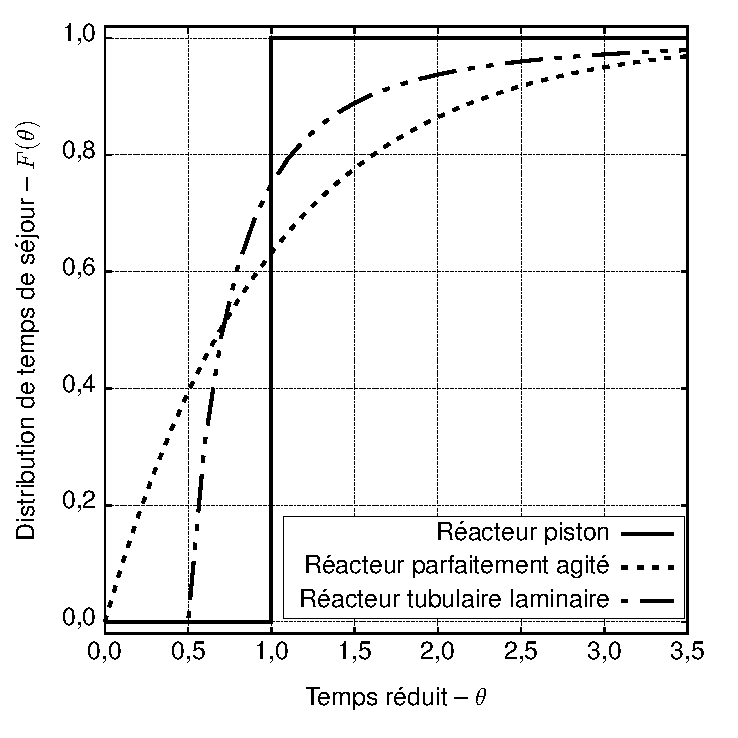
\includegraphics{figures/ch-01-types_de_reacteur}}
  
  \caption{\label{fig:types_de_reacteur}Distribution cumulative de temps de
    séjour en fonction du temps réduit pour différents types de réacteur.}
\end{figure}

\section{Cinétique des processus chimiques}
\label{sec:cinetique}

La connaissance précise du comportement de l'atmosphère carburante/nitrurante est fondamentale pour la maitrise industrielle des procédés thermochimiques.  Selon \citet{Dulcy2007} \og{}\textit{la compréhension des mécanismes de transfert de matière, des mécanismes physicochimiques associés à la réaction gaz-solide et des caractéristiques hydrodynamiques et thermiques des réacteurs a permis de concevoir des procédés permettant d'accroître la productivité par réduction des temps de traitement et corrélativement de réduire la consommation d'énergie}\fg{}.  L'optimisation des procédés thermochimiques est liée à la minimisation des résistances de transport de matière en phase gazeuse, au transfert de matière à l'interface gaz--solide et à l'intérieur du solide. Lorsque l'optimisation hydrodynamique est établie, dans le cas de la carbonitruration par exemple, il reste encore à diminuer la résistance à l'interface pour permettre la saturation de l'austénite en surface~\cite{Dulcy2007}, ce qui pour une nuance donnée représente l'optimum possible du transport à l'état solide.

Cela implique le besoin de traiter les réactions en phase gazeuse et aux interfaces gaz--solide \textendash{} parois du four et matériau traité \textendash{} afin d'améliorer la compréhension et donc le contrôle des mécanismes qui définissent la composition de l'atmosphère.  Un tel contrôle permettrait de prédire l'apport en carbone en fonction des paramètres opératoires du réacteur. Cette section présente les fondements théoriques de la cinétique chimique. Les systèmes cinétiques modélisés seront présentés avec les résultats expérimentaux au Chapitre~\ref{ch:modelisation_cinetique}.

Il faut remarquer que cette approche est valable lorsque le nombre de Knudsen~\cite{Hershey1973} $\varkappa=\nicefrac{\lambda}{L}$, où $\lambda$ est le libre parcours moyen et $L$ une dimension représentative de l'enceinte contenant le gaz, est inférieur à 0,01 \textendash{} donc dans un régime dit visqueux. À partir du moment où $\lambda$ est du même ordre de grandeur que les dimensions $L$ de l'enceinte contenant le gaz, les collisions moléculaires en phase homogène deviennent assez rares et les particules sont soumises principalement à des échanges de quantité de mouvement avec les parois du réacteur. Cette limite de régime possède deux implications fondamentales qui affectent fortement les traitements thermochimiques: comme le transport de masse et la cinétique chimique en domaine homogène dépendent des collisions entre les molécules, leur absence implique l'impossibilité de recourir aux équations des milieux continus pour modéliser le transport et toute modification de l'atmosphère résulte alors des interactions avec les surfaces catalytiques du réacteur. Pour les conditions que nous avons retenues pour la carbonitruration à basse pression (température de l'ordre de \SI{1173}{\kelvin} et pression de \SI{10}{\hecto\pascal}, dans des réacteurs ayant des dimensions de l'ordre de quelques dizaines de centimètres), on estime~\cite{Struchtrup2005} $\lambda\approx{10^{-5}}\ll{L}$ et donc le comportement du milieu peut être considéré comme continu, la description des mécanismes chimiques en phase homogène étant alors nécessaire.

\subsection{Processus homogènes: phase gazeuse}

La grande majorité des réactions chimiques ne donne pas lieu à une transformation directe des réactifs en produits finaux stables. Ces transitions s'opèrent par une série d'étapes intermédiaires faisant intervenir des états transitoires. Chacune de ces interactions est une réaction élémentaire~\cite{Green2007,Henriksen2008}. Un traitement détaillé des fondements physiques de ce sujet est disponible dans l'ouvrage de \citet{Henriksen2008}. Les réactions élémentaires conduisent en général à l'expression de lois de vitesse ayant des ordres entiers et identiques aux coefficients st{\oe}chiométriques des espèces participant à la réaction. Pour ce type de lois de vitesse dites élémentaires~\cite{Fogler1999}, les coefficients cinétiques possèdent un sens physique~\cite{Henriksen2008}.

Plusieurs logiciels et codes de simulation numérique existent pour fournir la solution de l'évolution de systèmes cinétiques chimiques. Même si plusieurs autres méthodes d'intégration de ces systèmes existent~\cite{Berberan1990, Park201342,Parumasur2005473,Bizetti2012}, on traitera la modélisation des réactions chimiques en phase gazeuse selon l'approche typique employée par la plupart des logiciels existant~\cite{Premix1998,Chemkin2000,Transport2000, SurfaceChemkin2000,Damian20021567,DetchemKin,Tchem2011,Cantera2014} dont le caractère général de la formulation est un avantage. Le problème se résume typiquement à résoudre un ensemble d'équations différentielles non--linéaires couplées, comprenant une équation pour chaque espèce chimique et une équation pour chaque variable thermodynamique indépendante. Étant donnés les écarts importants qu'il peut y avoir entre les échelles de temps pour les différents processus qui se déroulent simultanément, la solution numérique d'un tel système d'équations demande souvent l'emploi d'une méthode implicite~\cite{Coles2011} ou utilisant des intégrateurs à pas multiples, comme cela est proposé par les librairies Tchem~\cite{Tchem2011} et Cantera~\cite{Cantera2014} qui utilisent CVode~\cite{Hindmarsh2005}.

La description des vitesses de réaction adoptée dans le présent travail trouve ses fondements dans la loi d'action de masse~\cite{Landau1980}.  Cette formulation décrit l'équilibre chimique à travers des vitesses de processus directs et indirects qui doivent être les mêmes, permettant ainsi le calcul de la constante d'équilibre. Étant donnée la nature statistique de cette loi, les transformations sont dépendantes des pressions partielles \textendash{} \emph{i.e.} des quantités de matière \textendash{} des espèces participant à la réaction considérée. Pour introduire cette formulation, supposons une réaction élémentaire comme \ch{$\nu_{A}$ A + $\nu_{B}$ B <=> $\nu_{C}$ C + $\nu_{D}$ D}. La constante d'équilibre $K_{p}$ à une température donnée de cette réaction en termes de pressions partielles des espèces est fournie par l'Équation~\ref{eq:equilibrium_constant} qui la généralise. % en termes des coefficients st{\oe}chiométriques. %Le produit à droite dans cette expression, qui généralise la définition de $K_{p}$, laisse entendre implicitement que les coefficients st{\oe}chiométriques $\nu_{i}$ des réactifs sont de signe négatif et ceux des produits positifs. %Cela sera important plus tard quand on réalisera le bilan matière pour obtenir le taux d'avancement d'une réaction.

\begin{equation}
  K_{p}(T)=
  \frac{P_{C}^{\nu_{C}}P_{D}^{\nu_{D}}}{P_{A}^{\nu_{A}}P_{B}^{\nu_{B}}}=
  \prod_{i}P_{i}^{\nu_{i}}
  \label{eq:equilibrium_constant}
\end{equation}

Cette constante peut aussi être écrite en termes de concentrations des espèces à une pression totale $P$ donnée, ce que l'on note $K_{c}$ (Équation~\ref{eq:equilibrium_constant_concentration}).  Il faut remarquer que la dépendance de la constante d'équilibre $K_{c}$ avec la pression est liée au facteur $P^{-\sum\nu_{i}}$, où $\sum\nu_{i}$ représente le bilan molaire de la réaction. Considérons par exemple la décomposition de l'ammoniac, où $K_{c}\propto P^{-2}$, ce qui implique une augmentation de $K_{c}$ lorsque la pression est réduite. De l'équilibre des processus directs et indirects, une telle relation montre que la réduction de pression de \SI{1000}{\hecto\pascal} \textendash{} approximativement la pression atmosphérique \textendash{} à \SI{10}{\hecto\pascal}, typique des traitements thermochimiques à basse pression, mène à une réduction de quatre ordres de grandeur dans la quantité d'ammoniac disponible pour le traitement et donc à de possibles difficultés d'enrichissement en azote.

\begin{equation}
  K_{c}(T)=
  \big(P^{-\sum\nu_{i}}\big)K_{p}(T)=
  \prod_{i}c_{i}^{\nu_{i}}
  \label{eq:equilibrium_constant_concentration}
\end{equation}

On peut donc, à partir de la loi d'action de masse, introduire les taux d'avancement de réaction $\dot{\omega}$ dans chaque sens comme étant de la forme $\dot{\omega}=k\prod c_{i}^{\nu_{i}}$. La constante des processus directs sera notée $k_{f}$, celle des processus indirects $k_{b}$. Pour que la relation d'équilibre selon l'action de masse soit préservée, il faut que $K_{c}=\nicefrac{k_{f}}{k_{b}}$~\cite{Landau1980,Stolen2004}.  Une fois connue la constante cinétique d'un processus chimique, la thermodynamique fournit celle de la réaction indirecte \textemdash{} pour les processus réversibles. Ces constantes présentent, en général, une dépendance exponentielle avec la température qui peut être typiquement exprimée par une loi d'Arrhenius. Les données disponibles dans la littérature se trouvent le plus souvent exprimées sous forme de coefficients pour l'Équation~\ref{eq:reaction_constant}, où $A_{i}$ est le facteur pré--exponentiel lié au temps de vie moyen d'une espèce activée et à la fréquence de collision, $n_{i}$ est l'exposant de température et $E_{a,i}$ l'énergie d'activation, qui représente un seuil énergétique à dépasser pour activer la réaction.

\begin{equation}
  k_{f,i}=
  A_{i}{\biggr(\frac{T}{T_{ref}}\biggr)}^{n_{i}}\exp\left(-\frac{E_{a,i}}{RT}\right)
  \label{eq:reaction_constant}
\end{equation}

À partir de ces notions de processus directs et indirects et de la formulation de la loi d'action de masse en termes de concentrations, on peut écrire l'Équation~\ref{eq:advance_rate} pour le calcul des taux d'avancement de réaction. Cette équation est simplement le bilan entre les vitesses directes et indirectes des réactions.

\begin{equation}
  R_{i}=
  k_{f,i}\prod_{l=1}^{N_{s}}c_{l}^{\nu_{l,i}^{\prime}}-
  k_{b,i}\prod_{l=1}^{N_{s}}c_{l}^{\nu_{l,i}^{\prime\prime}}
  \label{eq:advance_rate}
\end{equation}

Finalement, en faisant le bilan molaire $\Delta{}\nu_{l}=\nu_{l,i}^{\prime\prime}-\nu_{l,i}^{\prime}$ pour l'espèce $l$ en fonction de ses coefficients st{\oe}chiométriques dans toutes les réactions où elle intervient comme produit ($\nu_{l,i}^{\prime\prime}$) et réactif ($\nu_{l,i}^{\prime}$), on obtient sa vitesse molaire de formation $\dot{\omega}_{l}$.  Cela est présenté dans l'Équation~\ref{eq:rate_species_general} qui introduit aussi le facteur $\mathbb{C}_{i}$. 

\begin{equation}
  \dot{\omega}_{l}=
  \sum_{i=1}^{N_{r}}\Delta{}\nu_{l}
  \mathbb{C}_{i}R_{i}
  \qquad\text{où}\qquad
  \mathbb{C}_{i}=
  \begin{cases}
    1 
    & \text{\footnotesize{}(i)}\\[8pt]
    \sum_{l=1}^{N_{s}}\alpha_{l,i}c_{l} 
    & \text{\footnotesize{}(ii)}\\[8pt]
    \dfrac{P_{r,i}}{1+P_{r,i}}F_{i} 
    & \text{\footnotesize{}(iii)}\\[8pt]
    \dfrac{1}{1+P_{r,i}}F_{i} 
    & \text{\footnotesize{}(iv)}
  \end{cases}
 \label{eq:rate_species_general}
\end{equation}

\clearpage

Ce facteur $\mathbb{C}_{i}$  introduit la dépendance avec la pression des processus chimiques. En général sa valeur est unitaire dans le cas (i) des réactions élémentaires \textemdash{} celles qui décrivent directement le processus chimique dans une seule étape. D'autres formulations sont présentées ci-dessous pour les réactions (ii) à trois corps, (iii) unimoléculaires et de récombinaison et (iv) bimoléculaires. % Ces descriptions supplémentaires sont nécessaires à la description des processus dont la formulation élémentaire n'est pas complètement connue ou quantifié~\cite{Green2007}.

Dans le cas d'une réaction simple, $\mathbb{C}_{i}$ est unitaire. Pour les réactions à trois corps, sa valeur représente la concentration effective du troisième corps, où $\alpha_{l,i}$ est l'efficacité du troisième corps pour l'espèce $l$ dans la réaction $i$ et $c_{l}$ sa concentration. Si toutes les espèces interviennent de manière équivalente en tant que troisième corps, les facteurs $\alpha_{l,i}$ sont tous unitaires et la concentration effective est la concentration du mélange.  Les processus de dissociation unimoléculaire et de récombinaison dépendent de la présence d'un troisième corps pour que le bilan énergétique soit possible. Selon la théorie de Lindemann, les vitesses de réaction sont proportionnelles à la concentration de ce troisième corps dans les systèmes dilués et arrivent à une valeur limite lorsque la concentration de ces espèces atteint un seuil.

Dans ce modèle de Lindemann, la pression réduite $P_{r,i}$ est définie par l'Équation~\ref{eq:reduced_pressure}. Par définition, l'efficacité du troisième corps $\alpha_{l,i}$ d'une espèce est unitaire. Si certaines espèces jouent un rôle sur la vitesse de réaction, seules les concentrations de ces espèces sont prises en compte par cette expression. Les constantes $k_{\infty,m}$ dans la limite des pressions élevées et $k_{0,m}$ dans la limite des pressions basses nécessaires à la description des réactions de types \og{}fall-off\fg{} et bimoléculaires activées chimiquement sont données comme des fonctions de la température selon l'Équation~\ref{eq:reaction_constant}. Dans le cas des réactions unimoléculaires et/ou de récombinaison, les paramètres d'Arrhenius de $k_{\infty,m}$ doivent être pris en compte pour le calcul de $k_{f,m}$. Pour les réactions bimoléculaires activées chimiquement, ce sont les valeurs de $k_{0,m}$ qui doivent être utilisées.

\begin{equation}
  P_{r,i}=\frac{k_{0,i}}{k_{\infty,i}}\sum_{k=1}^{N_{s}}\alpha_{l,i}c_{l}
  \label{eq:reduced_pressure}
\end{equation}

La transition entre les régimes de haute et basse pressions est modélisée par l'Équation~\ref{eq:falloff}, où les $a_{i}$, $T_{i}^{***}$, $T_{i}^{*}$ et $T_{i}^{**}$ sont des paramètres du modèle. Il existe d'autres formulations pour la modélisation de cette transition. Cependant, les mécanismes cinétiques employés dans le présent rapport utilisent les paramètres issus du formalisme de Troe.

\begin{equation}
  \log_{10}F_{i}=
  \biggr[1+\biggr(\frac{A}{B}\biggr)^{2}\biggr]^{-1}\log_{10}F_{cent,i}
  \label{eq:falloff}
\end{equation}

\noindent où les facteurs $F_{cent,i}$, $A$ et $B$ sont donnés par : 
\[
\begin{aligned} 
  & F_{cent,i}=
   (1-a_{i})\exp\biggr(-\frac{T}{T_{i}^{***}}\biggr)+
   a_{i}\exp\biggr(-\frac{T}{T_{i}^{*}}\biggr)+
   \exp\biggr(\frac{T_{i}^{**}}{T}\biggr)\\[5pt]
  & A=\log_{10}P_{r,i}-0,67\log_{10}F_{cent,i}-0,4\\[5pt]
  & B=0,806-1,1792\log_{10}F_{cent,i}-0,141\log_{10}P_{r,i}
\end{aligned}
\]

\clearpage

Étant donné le fait que les réactions s'accompagnent d'un changement de l'enthalpie libre du gaz ainsi que de sa masse molaire moyenne, laquelle intervient dans la concentration des espèces, l'ensemble des équations cinétiques ainsi écrites doit être fermé par une équation d'état. Cela se fait le plus souvent à l'aide de la loi des gaz parfaits donnée par l'Équation~\ref{eq:ideal_gas_law}.
%~\footnote{Les concentrations $c_{l}$ sont définies par le rapport entre le nombre de moles $N_{l}$ d'une espèce et le volume $V$ occupé par le système, $c_{l}=\nicefrac{N_{l}}{V}=\rho\nicefrac{Y_{l}}{M_{l}}$ -- où $\rho$ désigne la masse volumique et $Y_{l}$ la fraction massique relative à l'espèce de masse molaire $M_{l}$.}

\begin{equation}
  \rho=\frac{PM}{RT}\quad\text{où}\quad
  M=\sum_{i=1}^{N_{s}}X_{i}M_{i}=
  \biggr(\sum_{i=1}^{N_{s}}\frac{Y_{i}}{M_{i}}\biggr)^{-1}
  \label{eq:ideal_gas_law}
\end{equation}

Le changement de température dans le système est donné par l'Équation~\ref{eq:enthalpy_change}, où l'enthalpie molaire $h_{i}$ de l'espèce $i$ est calculée à partir d'un polynôme~\cite{Tchem2011}. Comme les procédés sont réalisés à pression constante, la dérivée de la pression au cours du temps est égale à zéro. Dans ce cas, si l'on simule un système fermé à volume variable, l'équation de la densité (ou du volume) doit être ajoutée au système d'équations différentielles à intégrer.

\begin{equation}
  \frac{\mathrm{d}T}{\mathrm{d}t}=
  -\frac{1}{\rho c_{p}}\sum_{i=1}^{N_{s}}h_{i}\dot{\omega}_{i}
  \label{eq:enthalpy_change}
\end{equation}

\subsection{Processus hétérogènes: interfaces solides}

Alors que la cinétique en phase gazeuse contrôle l'arrivée des précurseurs des traitements thermochimiques jusqu'aux surfaces des pièces à enrichir, ce sont les réactions hétérogènes qui apportent de la matière au solide. Cela n'est valable que si le nombre de Knudsen~\cite{Hershey1973} traduit un comportement visqueux, comme discuté au début de cette section. Sans quoi, la cinétique de surface gouverne le procédé. Ce n'est en général pas le cas à des pressions supérieures à \SI{1}{\hecto\pascal} comme cela a lieu dans les traitements de cémentation et de  nitruration des aciers. Par conséquent la compréhension des phénomènes d'enrichissement demande l'intégration simultanée des cinétiques homogènes et hétérogènes. Les vitesses des réactions hétérogènes doivent être proportionnelles aux flux nets des espèces participant aux réactions, lesquels sont orientés vers les surfaces. Cela comprend les flux par agitation thermique, diffusion, advection et accélération par des champs externes. En l'absence de champs, les vitesses des transports par advection et diffusion (de l'ordre de quelques \si{\metre\per\second})~\cite{Bird,Atkins2006} sont négligeables par rapport aux vitesses d'agitation thermique. On suppose donc que la vitesse de réaction ne dépend que de ce terme. La vitesse thermale moyenne $\bar{v}_{th}$ d'une espèce de masse molaire $M$ dans un gaz à température $T$ est donnée par l'Équation~\ref{eq:thermal_velocity}.

\begin{equation}
  \bar{v}_{th}=\biggr(\frac{8RT}{\pi{M}}\biggr)^{\nicefrac{1}{2}}
  \label{eq:thermal_velocity}
\end{equation}

L'Équation~\ref{eq:thermal_velocity} met en évidence une plus grande mobilité des espèces légères et donc l'influence plus prononcée de ces espèces sur les processus hétérogènes. On peut montrer à partir de la mécanique statistique~\cite{Atkins2006} que le flux $J_{i}$ d'une espèce $i$ par unité de surface est donné par l'Équation~\ref{eq:surface_flux}, où $\mathcal{N}_{i}$ désigne la concentration des molécules. Il est intéressant de noter dans cette formulation que l'effet de la température sur la masse volumique du gaz est prépondérant par rapport à son effet sur la vitesse moyenne des molécules.

\clearpage

\begin{equation}
  J_{i}=\frac{1}{4}\bar{v}_{th}\mathcal{N}_{i}=
  \frac{p_{i}N_{A}}{(2\pi{MRT})^{\nicefrac{1}{2}}}
  \label{eq:surface_flux}
\end{equation}

Ainsi, à basse pression partielle de précurseurs et à températures élevées, on doit s'attendre à que les flux d'espèces vers la surface soient faibles. Le taux d'adsorption dépend de la capacité du substrat à dissiper l'énergie de la particule arrivant; si la surface se trouve à haute température, il est très probable que l'adsorption n'ait pas lieu compte tenu des vibrations dans le solide. La probabilité d'adsorption, définie comme le rapport entre le taux d'adsorption et le flux de particules qui subissent une collision avec la surface reste faible. En outre, les processus de désorption ont des temps caractéristiques de l'ordre de \SIrange{10}{100}{\femto\second} et donc, la probabilité de recombinaison par diffusion en surface des espèces sorbées reste très faible ainsi que le taux de couverture $\theta$ de l'interface~\cite{Atkins2006}. Par conséquent, la contribution des processus de surface au changement de la composition dans le volume $V$ de l'atmosphère peut être exprimée globalement comme étant proportionnelle au flux des réactifs selon l'Équation~\ref{eq:rate_surface}, où $k_{w}$ désigne la constante de réaction et $S$ la surface traitée. 

\begin{equation}
V\frac{\mathrm{d}c_i}{\mathrm{d}t}=-k_{w}S{J_{i}}
\label{eq:rate_surface}
\end{equation}

Cette formulation suppose que le nombre de sites réactifs est intégré dans la constante de réaction $k_{w}$. En outre, comme les traitements étudiés ici sont réalisés sur des surfaces polycristallines sans orientation préférentielle, cette constante n'est qu'une moyenne globale sans aucun sens physique. Dans le cas plus général et complet de la description des processus de surface, différents types de sites sont disponibles pour les réactions hétérogènes en fonction des différents plans cristallins du matériau traité~\cite{Alcock2001}. 

Il faut remarquer qu'une telle description de processus traités de manière globale implique l'existence d'une température optimale au--delà de laquelle l'enrichissement des matériaux par voie thermochimique n'est pas favorable en raison de limitations cinétiques de surface: le transfert de matière est limité par le faible degré d'adsorption et par des conditions favorables à la désorption. Dans le cas des traitements à basse pression pour lesquels les temps de séjour dans l'enceinte du four deviennent assez courts, la conversion des précurseurs en phase gazeuse sera limitée, ce qui peut être à l'origine de difficultés d'enrichissement des surfaces.% traitées.  

\subsection{Simplification des mécanismes cinétiques}
\label{sec:simplification_cinetique_lu_and_law}

Comme cela a été défini tout au début de cette section, les processus chimiques élémentaires portent des informations relatives à la physique du système, tout en gardant aussi les relations d'interdépendance entre les espèces: les étapes élémentaires de réaction passant par des états de transition sont ainsi représentées.  En général, les mécanismes élémentaires comprennent des centaines ou même des milliers d'espèces chimiques, ce qui conduit à des ensembles de réactions de tailles similaires. Quelques exemples sont donnés par \citet{Coles2011}. Comme chaque espèce évolue au cours du temps, la modélisation en régime transitoire des écoulements réactifs \textendash{} comme c'est le cas pour les traitements thermochimiques à basse pression pendant toute la durée du traitement \textendash{} requiert d'ajouter une équation par espèce au système à résoudre.  Cela se fait le plus souvent en utilisant la méthode CFD~\footnote{De l'Anglais \textit{Computational Fluid Dynamics}.}~\cite{Liang2009} et plus récemment à l'aide de la méthode dite de Boltzmann sur réseau~\cite{Li20131194,Sullivan2006206} (LBM). Étant donné le grand nombre d'espèces typiquement présentes dans les modèles cinétiques détaillés, comme celui de \citet{Norinaga2009}, ces simulations sont généralement limitées en termes de temps de calcul, même avec les ordinateurs disponibles aujourd'hui. 

La modélisation de la pyrolyse et de la combustion des hydrocarbures atteint facilement des centaines, voire des milliers de réactions. Un mécanisme offrant une grande précision pour des courts temps de séjour et relatif à la pyrolyse 
%\textendash{} décomposition homogène \textendash{}
de l'acétylène a été proposé dans la littérature par \citet{Norinaga2007,Norinaga2007ii}.  Il a été validé expérimentalement par \citet{Norinaga2005} puis amélioré pour inclure des espèces de hauts poids moléculaires~\cite{Norinaga2009} pour arriver finalement à plus de 240 espèces et 900 réactions. La simulation directe d'écoulements réactifs qui inclurait un modèle aussi complet de la phase gazeuse n'est pas possible. Il faut tout d'abord obtenir une version simplifiée du schéma cinétique en ne gardant que les espèces du système présentant un intérêt pour l'application recherchée. Aucune méthode existant ne permet l'obtention d'un tel \og{}squelette\fg{} de mécanismes pour n'importe quel ensemble de conditions initiales. Dans le cas du système \ch{N-H} pour l'ammoniac, le mécanisme~\cite{Dirtu2006,Odochian2011} adopté est suffisamment simple pour être utilisé dans des calculs de CFD.

Avant de décrire la méthode de simplification adoptée pour inclure un modèle cinétique simplifié dans une simulation d'écoulement réactif, il convient de comprendre la différence entre réduction et simplification des modèles cinétiques. La réduction consiste en une procédure mathématique de diminution de la rigidité du système d'équations des espèces et des variables thermodynamiques considérées, rendant la solution du problème plus stable et convergente. Pour l'obtention des mécanismes squelettes, on parle de simplification : cela consiste à diminuer le nombre d'espèces et de réactions du système, en gardant les espèces majoritaires \textendash{} dont la connaissance préalable du comportement empirique lors de la pyrolyse est requise \textendash{} et celles aussi qui sont en forte interaction avec les espèces majoritaires~\cite{Coles2011}.

Plusieurs méthodes de simplification existent, comme l'analyse de sensibilité de \citet{Turanyi1989} et les hypothèses classiques des états quasi--stationnaires et d'équilibre partiel. Une comparaison entre plusieurs méthodes existantes a été effectuée par \citet{Coles2011}.  Dans le présent travail, on se limitera aux développements conduits par \citet{Lu2005} et aux applications et/ou améliorations proposées~\cite{Lu2006i,Lu2006ii,Pepiot2008}.  Ces méthodes ont comme caractéristique commune le besoin d'une connaissance préalable du comportement chimique du système. Plus récemment \citet{Curtis2015} ont proposé une implémentation à partir de la méthode de \citet{Pepiot2008} avec une sélection automatique des espèces. En outre, la méthode DRG~\footnote{De l'Anglais, Directed Relational Graph method.} de \citet{Lu2005} est très simple  à implémenter numériquement comparée à celle (CSP~\footnote{De l'Anglais, Computational Singular Perturbation method.}) de \citet{Lam1993,Lam1994}. Une utilisation de cette méthode dite des graphes de liaisons orientés de \citet{Lu2005} pour des simulations CFD est présentée par \citet{Liang2009} et s'avère satisfaisante.  La méthode de perturbation CSP de \citet{Lam1994} est utilisée avec succès par \citet{Ortega2007}. Une approche modifiée par \citet{Curtis2015} permet l'obtention automatique de mécanismes simplifiés en simulation avec une chimie adaptative.

\clearpage

La méthode~\cite{Lu2005} consiste en la construction d'un graphe de liaisons orientées entre espèces placées aux n{\oe}uds du graphe et les arêtes sont affectées d'un coefficient d'interaction $r_{ij}$ relatif aux espèces connectées ($i\rightarrow j$). Les ouvrages de \citet{Bondy1976} et \citet{Diestel2000} présentent des aspects de la théorie des graphes et de l'algorithme de recherche utilisé dans la méthode de simplification adoptée. Du fait que l'on considère le graphe orienté la matrice d'adjacence n'est pas symétrique, $r_{ij}\neq r_{ji}$, \textit{i.e.} l'espèce $i$ intervient sur la vitesse de formation de $j$ d'une manière différente de celle dont $j$ affecte $i$. Ce coefficient d'interaction $r_{ij}$ représente l'erreur sur le taux de formation de $j$ si l'on supprime $i$ du mécanisme et est défini par l'Équation~\ref{eq:coefficient_interaction}, où les paramètres ont les définitions fournies section précédente.  Le symbole de Kronecker $\delta_{jk}$ vaut l'unité si l'espèce $j$ est présente dans la réaction $k$ et zéro autrement.

\begin{equation}
  r_{ij}\equiv
  \dfrac{
   \sum_{k}^{N_{s}}\vert\nu_{i,k}\omega_{i}\delta_{jk}\vert}{
   \sum_{k}^{N_{s}}\vert\nu_{i,k}\omega_{i}\vert}
  \label{eq:coefficient_interaction}
\end{equation}

Si la valeur du coefficient est plus grande qu'un certain $\varepsilon$ défini avant la réduction, la suppression de $j$ du mécanisme produit un effet non--négligeable sur $i$. Donc, si $i$ doit être conservé dans le mécanisme, $j$ doit l'être aussi. En suivant cette logique, un graphe du système est construit de telle façon que l'arête $i\rightarrow j$ n'existe que si $r_{ij}\geq\varepsilon$. Une fois le graphe établi, on s'en sert comme algorithme de parcours en profondeur en partant des n{\oe}uds qui représentent les espèces choisies préalablement. Toutes les espèces retrouvées au cours de ce parcours sur le graphe sont retenues dans le mécanisme simplifié. Après identification de cet ensemble d'espèces, on élimine les réactions contenant d'autres espèces que celles retenues dans l'étape précedente. De cette façon, on obtient ainsi un mécanisme squelette. Il faut remarquer que le choix de $\varepsilon$ joue un rôle important sur la précision du mécanisme squelette. L'intersection de plusieurs réductions dans l'espace des états connus empiriquement produit des mécanismes avec une précision supérieure mais présentant l'inconvénient d'agréger plus d'espèces. Cette approche sera employée Chapitre~\ref{ch:modelisation_cinetique} pour l'obtention des mécanismes simplifiés à partir du mécanisme général de \citet{Norinaga2009}.

\clearpage\section{Conclusion}

Le Chapitre~\ref{ch:aspects_procedes} fait le point sur les aspects procédés liés aux traitements thermochimiques des aciers faiblement alliés. Les fondements qui y sont présentés servent de base aux discussions qui seront conduites dans les Chapitres~\ref{ch:caracterisation_atmospheres}~et~\ref{ch:modelisation_cinetique} et peuvent être résumés ainsi:
\begin{itemize}
  \item le contrôle des procédés de cémentation utilisant \ch{CO-H2} peut être réalisé à partir de diagrammes de températures de point de rosée. C'est aussi le cas pour les procédés de nitruration grâce aux diagrammes de potentiel de nitruration. Ces expressions sont disponibles pour le fer. Cette démarche peut être généralisée en utilisant la thermodynamique numérique;
  
  \item la diffusion du carbone et de l'azote à l'état solide dans des alliages à base de fer dépend des interactions entre les interstitiels et leur environnement métallurgique. Pour les systèmes plus simples, l'introduction d'une dépendance des coefficients de diffusion avec la composition peut être adoptée, mais pour les alliages \og{}réels\fg{}, l'approche formelle d'\citet{Onsager1931,Onsager1931ii} est nécessaire;
  
  \item la maîtrise des conditions aux limites pour les enrichissements en carbone et en azote nécessite un contrôle précis de l'atmosphère de traitement. Comme il n'est pas toujours possible de modéliser les réacteurs industriels par des approches limites de type réacteur \og{}agité\fg{} ou réacteur \og{}piston\fg{}, des mesures de la distribution de temps de séjour peuvent être utilisées pour prédire le degré de conversion des précurseurs dans les chambres de traitement;
  
  \item pour un suivi précis des atmosphères que l'on peut décrire comme des milieux continus, la modélisation de la cinétique détaillée doit être réalisée de manière couplée à l'écoulement et aux échanges thermiques dans le réacteur. Bien que cette approche permette le calcul du bilan énergétique interne grâce aux étapes élémentaires de la chaine de réactions, \emph{i.e} il possède une cohérence thermodynamique, son utilisation pour le suivi en temps réel et mise au point des réacteurs industriels est limitée par le grande nombre d'espèces et de réactions à considérer, ce qui couplé à la mécanique des fluides impose une contrainte en termes de temps de calcul. L'obtention de mécanismes simplifiés permet donc d'échantillonner l'ensemble des réactions et des espèces qu'il convient de retenir pour une région spécifique de l'espace des états et donc de réaliser des simulations de réacteurs réels dans un délai raisonnable pour des applications industrielles.  
\end{itemize}

\endinput